\documentclass{ipgplicence}
% Package pour personnaliser en-têtes et pieds de page
\usepackage{fancyhdr}
\usepackage{minted}
\usepackage{dirtree}
\usepackage{caption}
\usepackage{graphicx}
\usepackage{subcaption}
\usepackage[version=4]{mhchem}
\usepackage{listings}
\usepackage[most]{tcolorbox}
\usepackage[x11names]{xcolor}
\usepackage[table]{xcolor}
\usepackage{enumitem}
\setlist[itemize]{label=\color{ipgpred}$\blacktriangleright$}
\usepackage{booktabs}
\lstdefinestyle{mystyle}{
    backgroundcolor=\color{Snow1},
    breakatwhitespace=false,
    commentstyle=\color{gray},
    keywordstyle=\color{Green4},
    numberstyle=\footnotesize\color{gray},
    stringstyle=\color{purple},
    identifierstyle=\color{SteelBlue4},
    basicstyle=\ttfamily\small,
    numbers=left,
    keepspaces=false,
    numbers=left,
    showspaces=false,
    showstringspaces=true,
    breaklines=true,
    escapeinside={\%*}{*)},
    inputencoding = utf8,  % Input encoding
    extendedchars = true,  % Extended ASCII
    literate      =        % Support additional characters
      {á}{{\'a}}1  {é}{{\'e}}1  {í}{{\'i}}1 {ó}{{\'o}}1  {ú}{{\'u}}1
      {Á}{{\'A}}1  {É}{{\'E}}1  {Í}{{\'I}}1 {Ó}{{\'O}}1  {Ú}{{\'U}}1
      {à}{{\`a}}1  {è}{{\`e}}1  {ì}{{\`i}}1 {ò}{{\`o}}1  {ù}{{\`u}}1
      {À}{{\`A}}1  {È}{{\'E}}1  {Ì}{{\`I}}1 {Ò}{{\`O}}1  {Ù}{{\`U}}1
      {ä}{{\"a}}1  {ë}{{\"e}}1  {ï}{{\"i}}1 {ö}{{\"o}}1  {ü}{{\"u}}1
      {Ä}{{\"A}}1  {Ë}{{\"E}}1  {Ï}{{\"I}}1 {Ö}{{\"O}}1  {Ü}{{\"U}}1
      {â}{{\^a}}1  {ê}{{\^e}}1  {î}{{\^i}}1 {ô}{{\^o}}1  {û}{{\^u}}1
      {Â}{{\^A}}1  {Ê}{{\^E}}1  {Î}{{\^I}}1 {Ô}{{\^O}}1  {Û}{{\^U}}1
      {œ}{{\oe}}1  {Œ}{{\OE}}1  {æ}{{\ae}}1 {Æ}{{\AE}}1  {ß}{{\ss}}1
      {ç}{{\c c}}1 {Ç}{{\c C}}1 {ø}{{\o}}1  {Ø}{{\O}}1   {å}{{\r a}}1
      {Å}{{\r A}}1 {ã}{{\~a}}1  {õ}{{\~o}}1 {Ã}{{\~A}}1  {Õ}{{\~O}}1
      {ñ}{{\~n}}1  {Ñ}{{\~N}}1  {¿}{{?`}}1  {¡}{{!`}}1
      {°}{{\textdegree}}1 {º}{{\textordmasculine}}1 {ª}{{\textordfeminine}}1
    }

\renewcommand{\labelitemi}{\color{ipgpred}$\blacktriangleright$}

\definecolor{ipgpred}{RGB}{164, 22, 35}
\definecolor{ipgpdark}{RGB}{90, 10, 18}
\definecolor{ipgpgray}{RGB}{245, 245, 245}

\begin{document}

\pagecolor{ipgpred}   % ← fond rouge sur toute la page
\color{white}         

\vspace*{6cm}

\begin{center}
\colorbox{white}{%
  \parbox{\textwidth}{%
    \centering
    \color{ipgpred}
    \vspace{1.5cm}
    {\Huge\bfseries Manuel d'utilisation}\\[0.5em]
    {\LARGE SAFE-M-ORP}\\
    \vspace{1cm}
    {\large\itshape Juillet 2026}\\[1em]
    {\large\itshape Mathis Velasco et François Métivier, IPGP}\\[1em]
    {\large\itshape \textit{Avec la participation de :}\\
M. Velasco, P. Martin, A. Levasseur, A. Boubakour, H. Ast, R. Godard-Galves,
 I Or.lovic, S. Maurice, I. Piketty, L. Avney-On, 
 I. Ferrand, A.Faura (2026) }\\[1em]
    
    \vspace{1.5cm}
  }%
}%
\end{center}



\newpage

\pagestyle{fancy}



\section*{Résumé}

\pagecolor{white}\color{black}
\section*{Manuel à destination de l’utilisateur}

Ce Potentiomètre est simple d’utilisation pour la mesure d'ORP (\textit{Oxidation Reduction Potential}). Il est aisé de naviguer dans l’interface avec
un système simple de question-réponse, qui nécessite un ordinateur pour utiliser le code et envoyer
les informations. Les procédures d’étalonnage sont très simples et peuvent être réalisées pour une ou
deux solutions tampons.
La sonde ORP est confiné dans son étui de protection qui lui permet d’être facilement déplacé.\\

\tableofcontents
\newpage


\section{Installation de l'appareil et du programme}

\subsection{Técharger le projet SAFE-M-ORP}
Le programme du pH mètre est en accès libre sur le site internet github sur le compte ‘fme-
tivier’ \url{https://github.com/SAFE-M/SAFE-M-ORP-}. Un moyen simple de le trouver est de taper ‘github
fmetivier’ dans la barre de recherche. Une fois sur la page du profil de fmetivier, cliquez sur reposi-
tories. Une fois cela fait il faut alors cliquer sur le dossier du nom ‘SAFE-M-ORP’. Puis, en haut à
gauche cliquez sur le bouton vert ‘code’ et copier le lien github du dossier. Ensuite dans le terminal
(Ctrl+Alt+T pour l’ouvrir) saississez :
\begin{center}
\begin{verbatim}
  git clone https://github.com/SAFE-M/SAFE-M-ORP.git
\end{verbatim}
\end{center}
\subsection{Description fonctionnelle}

La figure \ref{boitier} montre le boîtier SAFE-M-ORP composé de :
\begin{enumerate}
    \item Sonde température PT100
    \item Sonde ORP
    \item Prise et branchement d’alimentation du Potentiomètre
\end{enumerate}


\begin{figure}[hbt]
\begin{center}
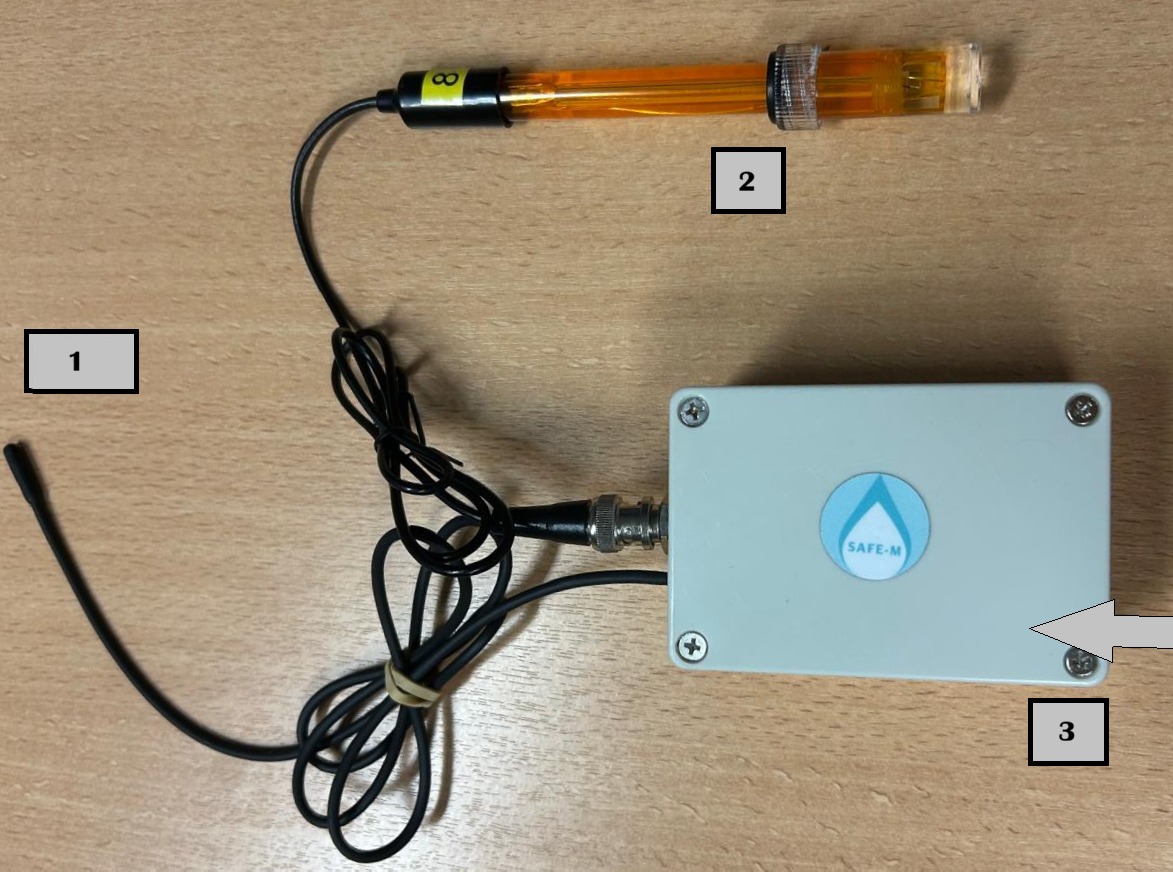
\includegraphics[width =0.7\textwidth]{figures/photo_boitier2.png}
\caption{Photographie du boîtier SAFE-M-ORP}
\label{boitier}
\end{center}
\end{figure}
\begin{figure}
\label{gitclone}
\end{figure}
\vspace{1cm}
\newpage
\begin{figure}
\begin{center}
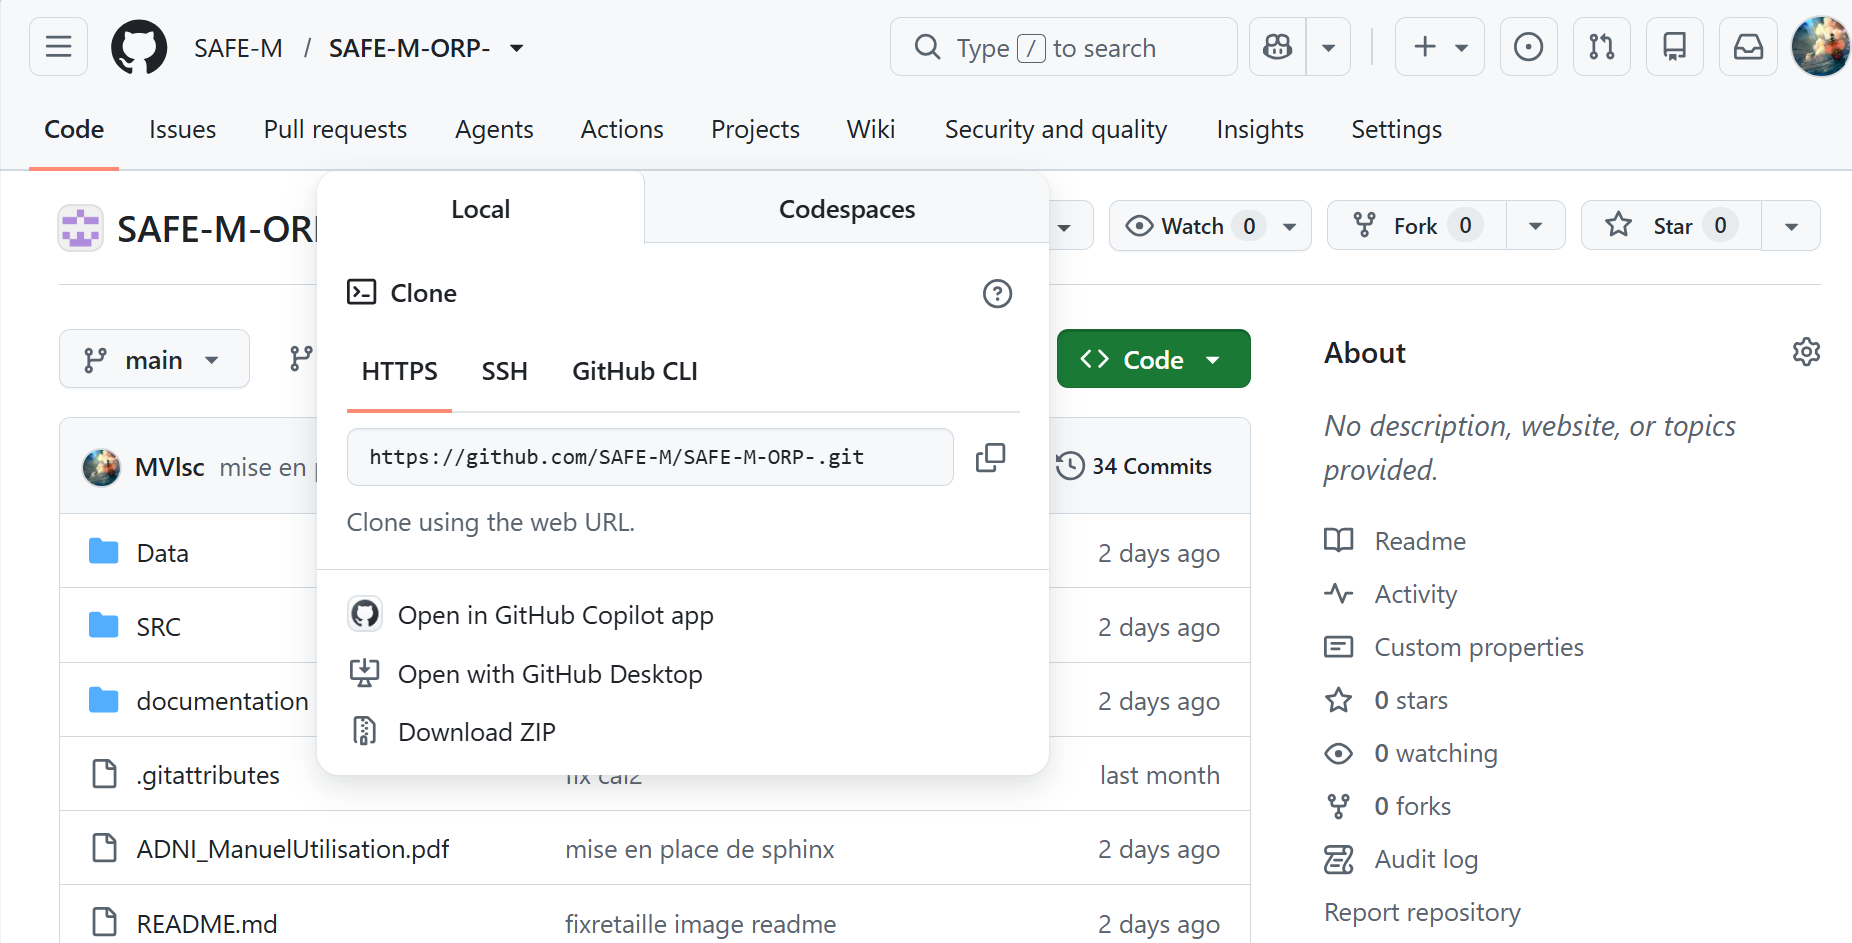
\includegraphics[width = 0.8\textwidth]{figures/git clone.png}
\caption{Copier/coller le lien en cliquant sur code.}
\end{center}
\end{figure}
Le dossier est alors chargé sur l’ordinateur de manière locale. Une fois le dossier chargé vous pouvez
vérifier le contenu du dossier en le comparant avec le dossier sur le site github. Le programme et toutes
ses composantes sont alors chargées, vous pouvez dès lors utiliser les pH-mètres.



\subsection{Matériel nécessaire à l'utilisation}

\begin{itemize}
    \item Boîtier
    \item Sonde ORP
    \item Solution étalon 
    \item Eau déminéralisé ou déionisée. 
    \item Bécher 
    \item Ordinateur + Réseau (pour l'installation du programme)
\end{itemize}
\newpage
\subsection{Connexion boîtier / Ordinateur}
Le code contenu dans le dossier "SRC/Mesure.py"  contient une fonction permettant d'établir la connexion série avec l'Arduino. L'utilisateur
peut choisir de fournir un port manuellement, sinon, grâce à une reconnaissance de nom de port, 
le programme va sélectionner automatiquement le nom relié à l'Arduino. 
Un filtre pour reconnaître les ports Linux ou Windows a été mis en place.


\section{Méthode Opératoire}
\subsection{Préparation initiale}
Avant de lancer le programme, branchez l'appareil avec le cable d’alimentation à un des ports USB
de l’ordinateur. Ensuite branchez la sonde ORP sur le boitier. Devissez le capuchon de la
sonde ORP. Rincez la sonde avec de l’eau distillée ou de l’eau claire si vous n’avez pas d’eau distillée
à votre disposition. Séchez puis plongez la Sonde ORP dans la solution à mesurer.

Ouvrez le terminal depuis le dossier SRC ou alors vous pouvez allez dans le terminal de votre ordinateur, placez vous dans le dossier avec la commande ‘cd’:
\begin{verbatim}
    cd "chemin/.../"SAFE-M-ORP"/"SRC"
\end{verbatim}

Saissisez ensuite la comande pour lancer le programme :\\
\textbf{Sur Linux :} \begin{verbatim}
    python3 'consigne.py'
\end{verbatim}
\textbf{Sur Windows:} \begin{verbatim}
    python 'consigne.py'
\end{verbatim}

\begin{tcolorbox}[colback=gray!20, colframe=gray]
    ATTENTION /!\textbackslash{} :\\
    La première ligne que renvoie le terminal affiche : 
\begin{verbatim}
#windows
    Connexion réussie sur COM(...)
#Linux :
    Connexion réussie sur ttyACM(...)
\end{verbatim}
Si il est affiché :\\
/!\textbackslash{} Aucun port Arduino détecté\\
Essayez de rebrancher les ports ou de l'indiquer manuellement.
\end{tcolorbox}

\begin{figure}
    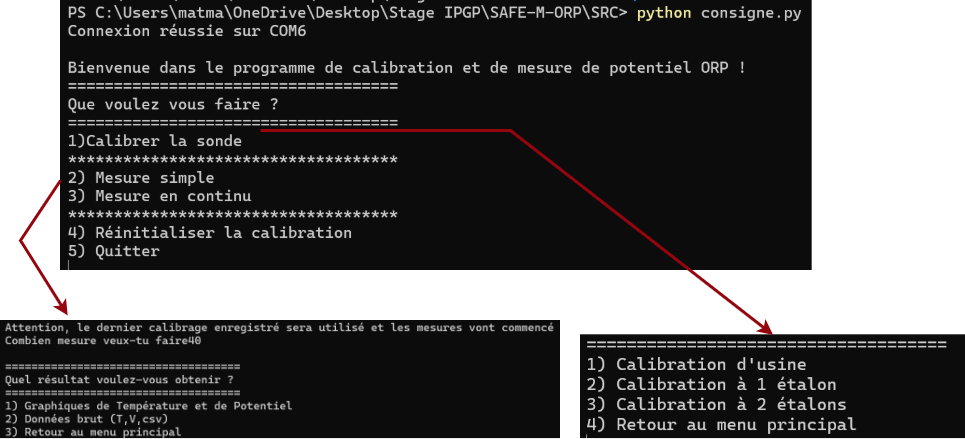
\includegraphics[width=0.7\textwidth]{figures/menu.png}
\caption{Menu principale avec deux exemples de sous-menu}
\label{menu}
\end{figure}

\newpage
\section{Calibration de l'appareil}
\label{cal}
\subsection{Etalonnage de la sonde ORP}
Pour une meilleure exactitude, un étalonnage fréquent de l’instrument est recommandé. Un étalonnage
est indispensable dans les cas suivants :
\begin{itemize}
 \item L’électrode (sonde ORP) ou le boîtier a été remplacée
 \item Au moins une fois par mois
 \item  Après avoir mesuré des produits chimiques agressifs
 \item  Lorsqu’une grande exactitude est requise
\end{itemize}
\subsection{Lancer la calibration}
Lancer le programme, taper 1, puis choissiez si vous souhaitez faire une calibration à 1,2 ou 0 étalons.
Suivez les consignes précisé dans le terminal. 

{\Large\textbf{Protocole :}}\\
\begin{itemize}
    \item Enlever le capuchon au KCl de la sonde... et calibrez votre sonde (voir \ref{cal})
    \item Rincer à l'eau distillé (ou propre) le bout de la sonde + sécher 
    \item Plongez dans la solution
    \item Attendez 10-20 secondes puis lancer la mesure
    \item Reproduire le protocole pour le deuxième étalon (pour la calibration à 2 étalons)
\end{itemize}
\begin{tcolorbox}[colback=gray!20, colframe=gray]
    {\Large\textcolor{orange}{Conseil}\\}
Pour la calibration, nous vous conseillons de commencer les mesures 
au moin 30 secondes après l'immersion de la sonde dans la solution, afin que les mesures soient stables ainsi
que de faire au choisir 100 mesures pour réduire au maximum l'écart type et avoir une moyenne précise.
\end{tcolorbox}
\begin{tcolorbox}[colback=gray!20, colframe=gray]
    {\Large\textcolor{red}{Important}\\}
Pour réaliser des mesures précises, il est préférable de connaître la plage de potentiel du milieu étudié avant 
toute calibration. L'influence d'une solution (voir rapport)de plus haut potentiel que le milieu sur les sondes 
suggère que la calibration à deux étalons est peu adaptée à ce type de mesure.
\end{tcolorbox}
L’étalonnage est maintenant terminé, vous pouvez commencer à effectuer vos mesures en retournant sur le menu d'acceuil.
\begin{tcolorbox}[colback=gray!20, colframe=gray]
    {\Large\textcolor{green}{Remarque}\\}
La calibration est enregistré une fois réalisé jusqu'a la prochaine calibration, pour réinitialiser la la calibration (=calibration d'usine)
appuyez sur 4 dans le menu principale
\end{tcolorbox}


\section{Mesures}
Après avoir mis en place la sonde ORP comme expliqué pour la calibration, il y a deux choix de mesure possible pour l'utilisateur : 

\begin{figure}[h]
    \centering
    \begin{subfigure}[b]{0.43\textwidth}
        \centering
        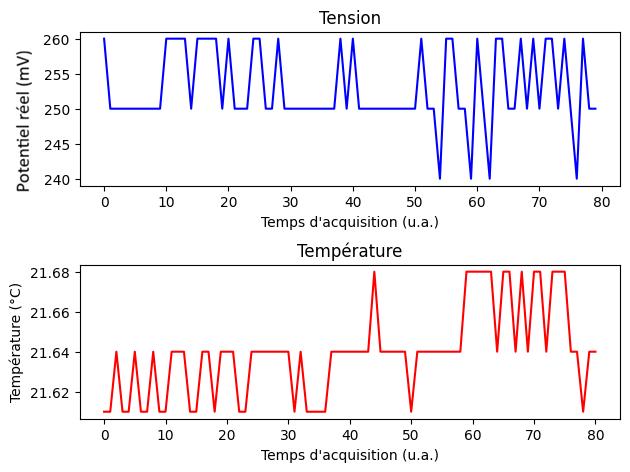
\includegraphics[width= 8cm]{figures/acqui2.png}
        \caption{}
        \label{fig:1a}
    \end{subfigure}
    \hfill
    \begin{subfigure}[b]{0.52\textwidth}
\includegraphics[width=12cm]{figures/acquI1.png}        
\caption{}
        \label{fig:1b}
    \end{subfigure}
    \caption{ (a) Acquisition en direct avec affichage des mesures, (b) Acquisition par nombre de mesures choisi }
\end{figure}

{\Large\textbf{Protocole :}}\\
\begin{itemize}
    \item Enlevez le capuchon au KCl de la sonde 
    \item Rincez à l'eau distillé (ou propre) le bout de la sonde + séchez 
    \item Plongez la sonde dans la solution
    \item Attendez 10-20 secondes puis lancer la mesure par méthode (a) et pour la méthode (b) attendre que la mesure se stabilise.
    \item Reproduire le protocole pour le deuxième étalon (pour la calibration à 2 étalons)
    \item Une fois les mesures finis, nettoyez votre sonde et remettez le bout de l'éléctrode dans son capuchon au KCl

\end{itemize}
 La méthode (a) permet de pouvoir voir quand la sonde est stabilisée pour éviter de prendre des données inutiles. 
Pour cela, il vous est indiquer :
\begin{verbatim}
    /!\\ Attention, le dernier calibrage enregistré sera utilisé.
Si vous souhaitez sauvegarder les données veillez à noter a partir du temps le potentiel se stabilise (en entier) ')
Les mesures commencent, pour arreter appuyez sur q
\end{verbatim}

Ainsi, si vous avez fait mesuré pendant 200s  et que la mesure de la sonde est stable au bout de 10, alors vous pouvez enregistré les 80 dernières secondes stables.
\begin{tcolorbox}[colback=gray!20, colframe=gray]   
    {\Large\textcolor{green}{Remarque}\\}
Si appuyer sur q ne ferme pas le graphique, cliquez sur le graphique et réappuyez sur q ( à plusieurs fois)
\end{tcolorbox}
 La méthode (b) demande moin de ressource pour l'ordinateur, plus pratique sur des PC peu puissants.
Après avoir choisi un chiffre de mesure (100 minimum conseillé) pour acquérir les données, vous pourrez sauvegardez vos données ou tracé un graphique, si vous 
tracez un graphique vous pourrez enregistrer les données par la suite aussi.


\begin{tcolorbox}[colback=gray!20, colframe=gray]   
    {\Large\textcolor{orange}{Conseil}\\}
Pour avoir des mesures précises, il est nécessaire
que l’instrument ait été étalonné au préalable. Si les mesures sont effectuées dans des échantillons
successifs, il est recommandé de rincer l’électrode entre chaque échantillon, afin de ne pas contaminer
les échantillons entre-eux.
\end{tcolorbox}
\vspace{-0.5 cm}
\section{Annexes}
\subsection{Organisation du code}
\label{code}
% Dans le document :
\dirtree{%
.1 SAFE-M-ORP.
.2 Data.
.3 data\_figures.
.3 data\_(T,V).
.3 data\_calibration.
.2 documentation.
.3 Documentation.md.
.3 Rapport\_SAFE-M-ORP.pdf.
.3 manuel.
.4 figures.
.4 manuel.tex.
.4 manuel.pdf.
.3 \_build.
.4 html.
.2 SRC.
.3 \_\_pycache\_\_.
.3 arduino\_redox.
.3 calibration.py.
.3 consigne.py.
.3 Mesure.py.
.2 .gitattributes.
.2 AUTHORS.md.
.2 LICENCE.rst.
.2 README.md.
}

Le projet SAFE-M-ORP est constitué en trois blocs principaux : 
\begin{enumerate}
    \item Le dossier Source (\textit{SRC}) où l'on retrouvera : 
    \begin{itemize}
        \item \textit{Mesure.py} qui contient toutes les fonctions pour permettre d'effectuer les mesures, les graphiques, les enregistrements et la connexion au port Arduino.
        \item \textit{calibration.py} qui contient les fonctions permettant un étalonnage d'usine, à 1 et 2 étalons ainsi que les fonctions pour enregistrer ces calibrations. 
        \item \textit{consigne.py} qui contient le menu interactif avec l'utilisateur lui permettant de choisir ce qu'il veut faire. 
        \item \textit{arduino\_redox.py} qui contient le code C/C++ à téléverser sur les cartes Arduino Uno pour  
        l'acquisition des mesures. 
        \item \textit{\_\_pycache\_\_} est un dossier généré automatiquement par Python qui contient les fichiers compilés (.pyc) des scripts.
    \end{itemize}

    \item Le dossier documentation :
    \begin{itemize}
        \item \textit{manuel} ou l'on y retrouve le manuel d'utilisation (\textit{pdf}) avec son document \textit{tex} et les figures nécessaires.
        \item \textit{Rapport\_SAFE-M-ORP} qui est un document détaillant le principe d'utilisation de la sonde ainsi que ses limitations.
        \item \textit{\_build} qui correspond aux outils sphinx seulement développer en \textit{html}
        \item \textit{Documentation.md} qui décrit le fonctionnement du programme.
    \end{itemize}

    \item Et le dossier Data qui contient les données des mesures (et calibration) sous la forme fichier \textit{.csv} ou des graphiques sous la forme \textit{.png}. 
    Les fichiers \textit{.csv} sont principalement organisés comme ci-dessous : 
\end{enumerate}
\begin{verbatim}
#Donnees Temperature / Potentiel(calibre), pour V :  écart type =5.74 et moyenne = 53.14
21.61,260.00
21.61,250.00
21.64,250.00
21.61,250.00
21.61,2
\end{verbatim}
\newpage
\section{Montage de l'appareil}
\begin{figure}[h]
    \centering
    \begin{subfigure}[b]{0.8\textwidth}
        \centering
        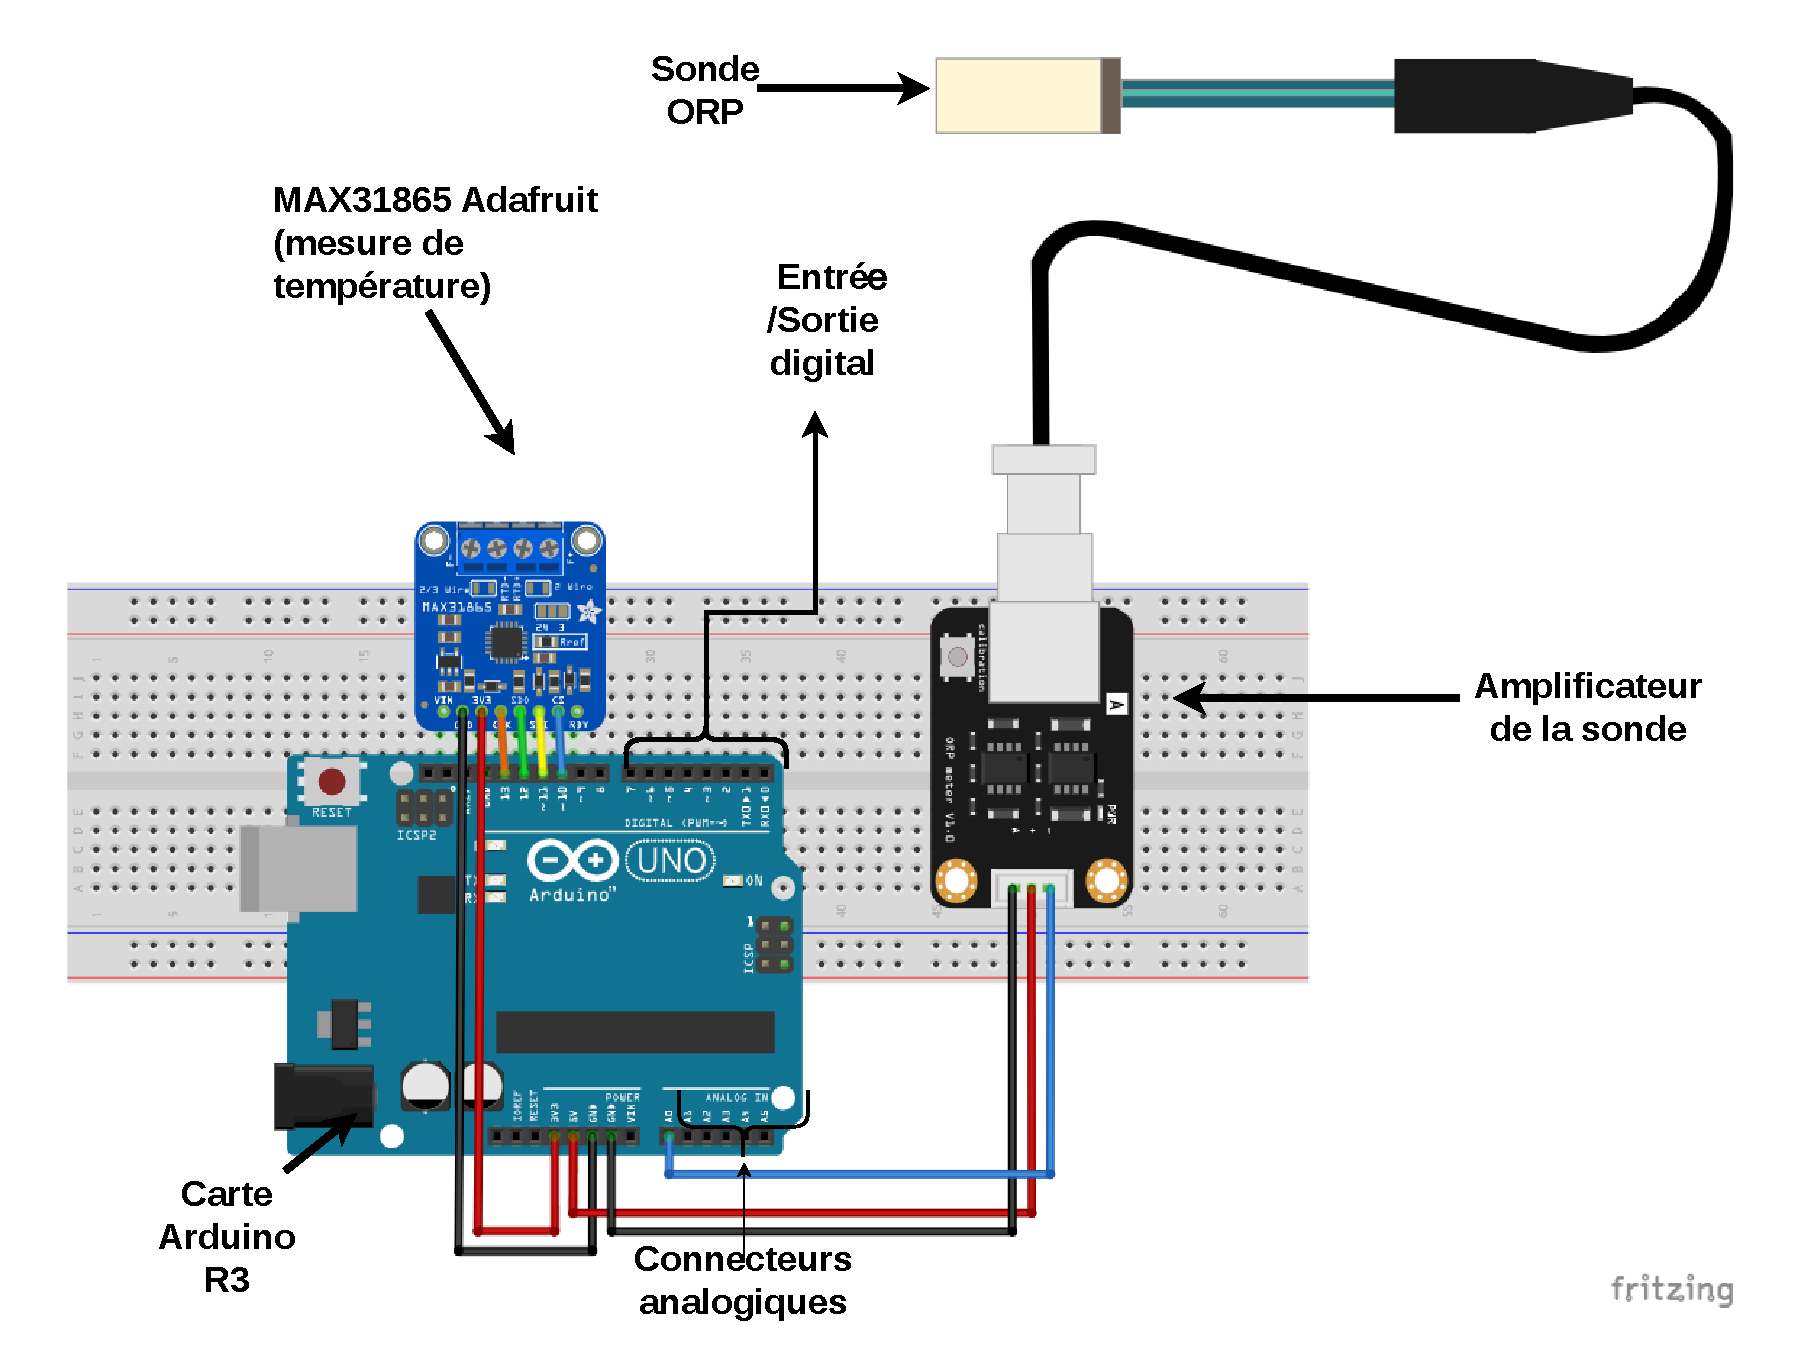
\includegraphics[width=\textwidth]{figures/montageArduino.pdf}
        \caption{}
        \label{fig:1a}
    \end{subfigure}
    \hspace{0.5 cm}
    \begin{subfigure}[b]{0.4\textwidth}
        \centering
        \begin{tabular}{c|c}
            \hline
            \rowcolor{ipgpred}
            \textbf{Port} & \textbf{Uno} \\
            \hline
            \hline
            SDI & 11 \\
            SDO & 12 \\
            CLK & 13 \\
            CS  & 10 \\
            \hline
        \end{tabular}
        \caption{}
        \label{fig:1b}
    \end{subfigure}
    \caption{(a) Montage Manuel de l'Arduino, (b) Connexions des ports analogiques à l'interface MAX31865 d'Adafruit.}
\end{figure}


\begin{tcolorbox}[colback=gray!20, colframe=gray]
    {\Large\textcolor{red}{Important}\\}
Pour pouvoir emboîter correctement la carte \textit{fritzing} sur la carte Arduino Uno, 
il faut veiller à souder par dessus celle ci, c'est à dire sur la même face que l'interface Adafruit.
\end{tcolorbox}

\end{document}